%-------------------------------------------------------------------------------
%                            BAB IV
%               		HASIL DAN PEMBAHASAN
%-------------------------------------------------------------------------------
\fancyhf{} 
 \fancyfoot[C]{\thepage}
\chapter{HASIL DAN PEMBAHASAN}


\section{Perancangan Sistem}

Tahap perancangan sistem ini meliputi perancangan alur kerja sistem yang berfungsi untuk memastikan sistem yang dibangun dapat digunakan secara baik oleh pengguna. Tahap perancangan sistem ini terbagi menjadi beberapa bagian yaitu diagram Use Case , Diagram Deployment, alur kerja sistem, \textit{Flow Diagram} dan desain prototipe berdasarkan analisa kebutuhan yang telah dijabarkan. Berikut ini merupakan tahapan tersebut:



\begin{enumerate}
\item \textit{Use Case Diagram}
\par \textit{Use Case Diagram} merupakan gambaran interaksi antara pengguna dan sistem. Pengguna dari sistem yang akan dibangun ini adalah Tunanetra dan pengunjung gedung FMIPA USK. \textit{Use Case Diagram} dari sistem ini dapat dilihat pada Gambar \ref{img:use_case_diagram}

\begin{figure}[H]
\centering
{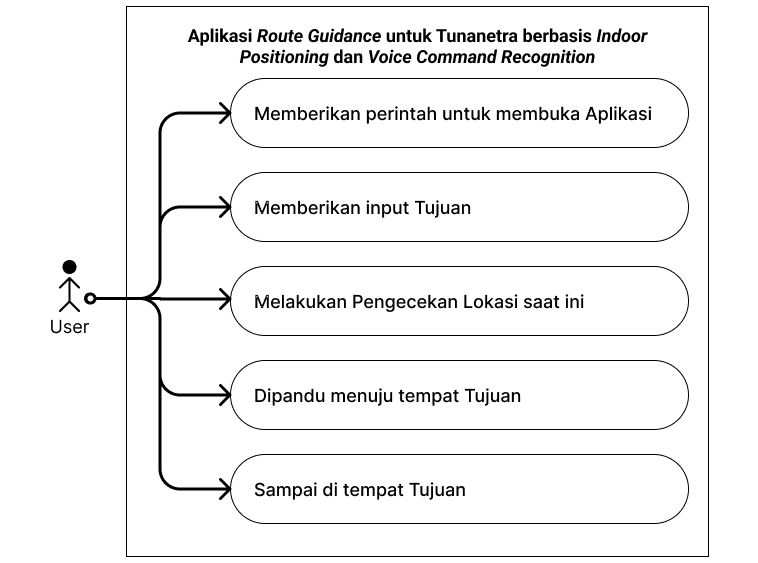
\includegraphics [width = 12cm, height= 10cm]{gambar/bab3/use_case_diagram}}
\caption{\textit{Use Case Diagram}}
\label{img:use_case_diagram}
\end{figure}

\newpage
\item \textit{Deployment Diagram}
\par \textit{Deployment Diagram} merupakan gambaran hubungan antara perangkat lunak dan perangkat keras yang digunakan dalam sebuah sistem. Seperti yang telah disebutkan sebelumnya, penelitian ini merupakan bagian dari penelitian lain yang saling terintegrasi sehingga tidak semua \textit{node} dalam diagram menjadi fokus dalam penelitian ini. Bagian dalam diagram yang menjadi jangkauan dari penelitian ini ditandai dengan warna biru seperti yang ditunjukkan pada Gambar \ref{img:deployment_diagram}

\begin{figure}[H]
\centering
{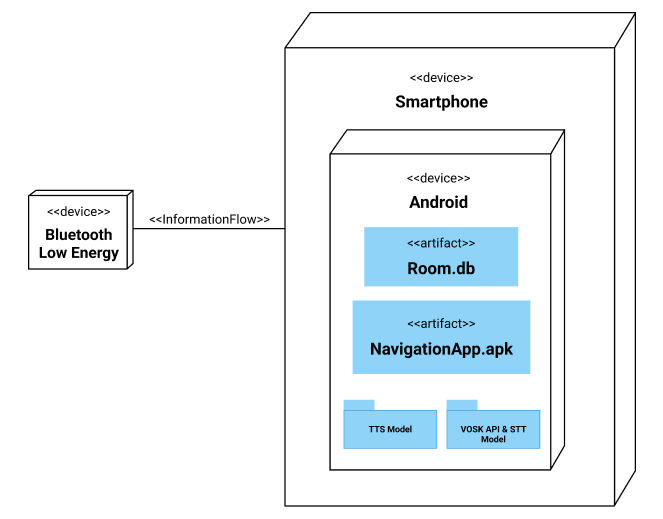
\includegraphics [width = 8cm, height= 6cm]{gambar/bab3/deployment_diagram}}
\caption{\textit{Deployment Diagram}}
\label{img:deployment_diagram}
\end{figure}

\newpage

\item \textit{Class Diagram}
\par \textit{Class Diagram} merupakan gambaran struktur sistem untuk memodelkan sistem mulai dari kelas sistem, atribut, metode dan hubungan antar objek. fungsi utama \textit{class diagram} adalah untuk memvisualisasikan, menentukan, dan mendokumentasikan fitur struktural dari pemodelan sistem, dalam penelitian untuk BLE Data yang akan disimpan secara lokal dalam \textit{database}. Berikut adalah \textit{class diagram} untuk penelitian ini.

\begin{figure}[H]
\centering
{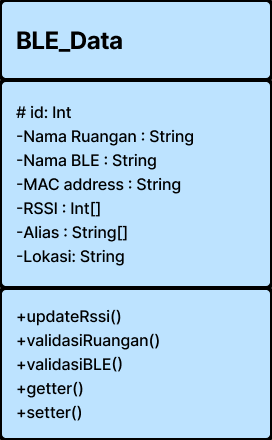
\includegraphics [scale = 0.5]{gambar/bab4/Class-Diagram}}
\caption{\textit{Class Diagram}}
\label{img:class_diagram}
\end{figure}

\newpage


\item Alur Kerja Sistem

\par Alur kerja sistem merupakan langkah-langkah yang dilalui sistem hingga fungsionalitas sistem dapat dimanfaatkan oleh pengguna. Alur kerja sistem ini dapat dilihat pada Gambar \ref{img:alur_kerja_sistem}

\begin{figure}[H]
\centering
{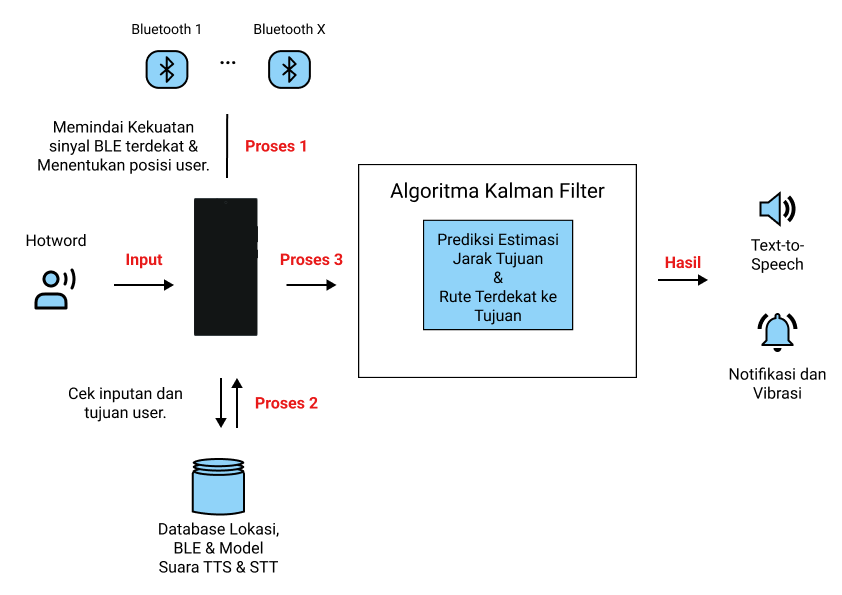
\includegraphics [scale = 0.5]{gambar/bab3/alur_kerja_sistem}}
\caption{Alur Kerja Sistem}
\label{img:alur_kerja_sistem}
\end{figure}

\begin{itemize}
\item \textit{Input} diterima dari pengguna setelah mengucapkan \textit{hotword}.

\item Pada proses 1 aplikasi dan perangkat akan memindai kekuatan sinyal BLE terdekat serta menentukan posisi pengguna.

\item Pada proses 2, setelah posisi pengguna ditentukan, aplikasi akan melakukan pengecekan \textit{input} dari pengguna pada \textit{database} lokasi menggunakan model yang telah tersedia oleh penelitian lainnya.

\item Pada proses 3, aplikasi akan memprediksi jarak tujuan serta rute terdekat menuju tujuan pengguna menggunakan algoritma Kalman Filter.

\item Hasil yang dihasilkan dari proses-proses sebelumnya berupa notifikasi dan vibrasi serta \textit{text-to-speech} atau berupa ucapan dari rute yang akan di tempuh oleh pengguna, seperti "Belok ke kanan dalam 5 langkah", "Telah sampai di tujuan , Ruangan Jurusan Informatika", dsb.
\end{itemize}

\newpage
\item \textit{Flow Diagram}
\par \textit{Flow Diagram} menunjukkan bagaimana proses tahapan melakukan navigasi pada sistem seperti pada gambar \ref{img:flow_diagram_app} berikut ini.

\begin{figure}[H]
\centering
{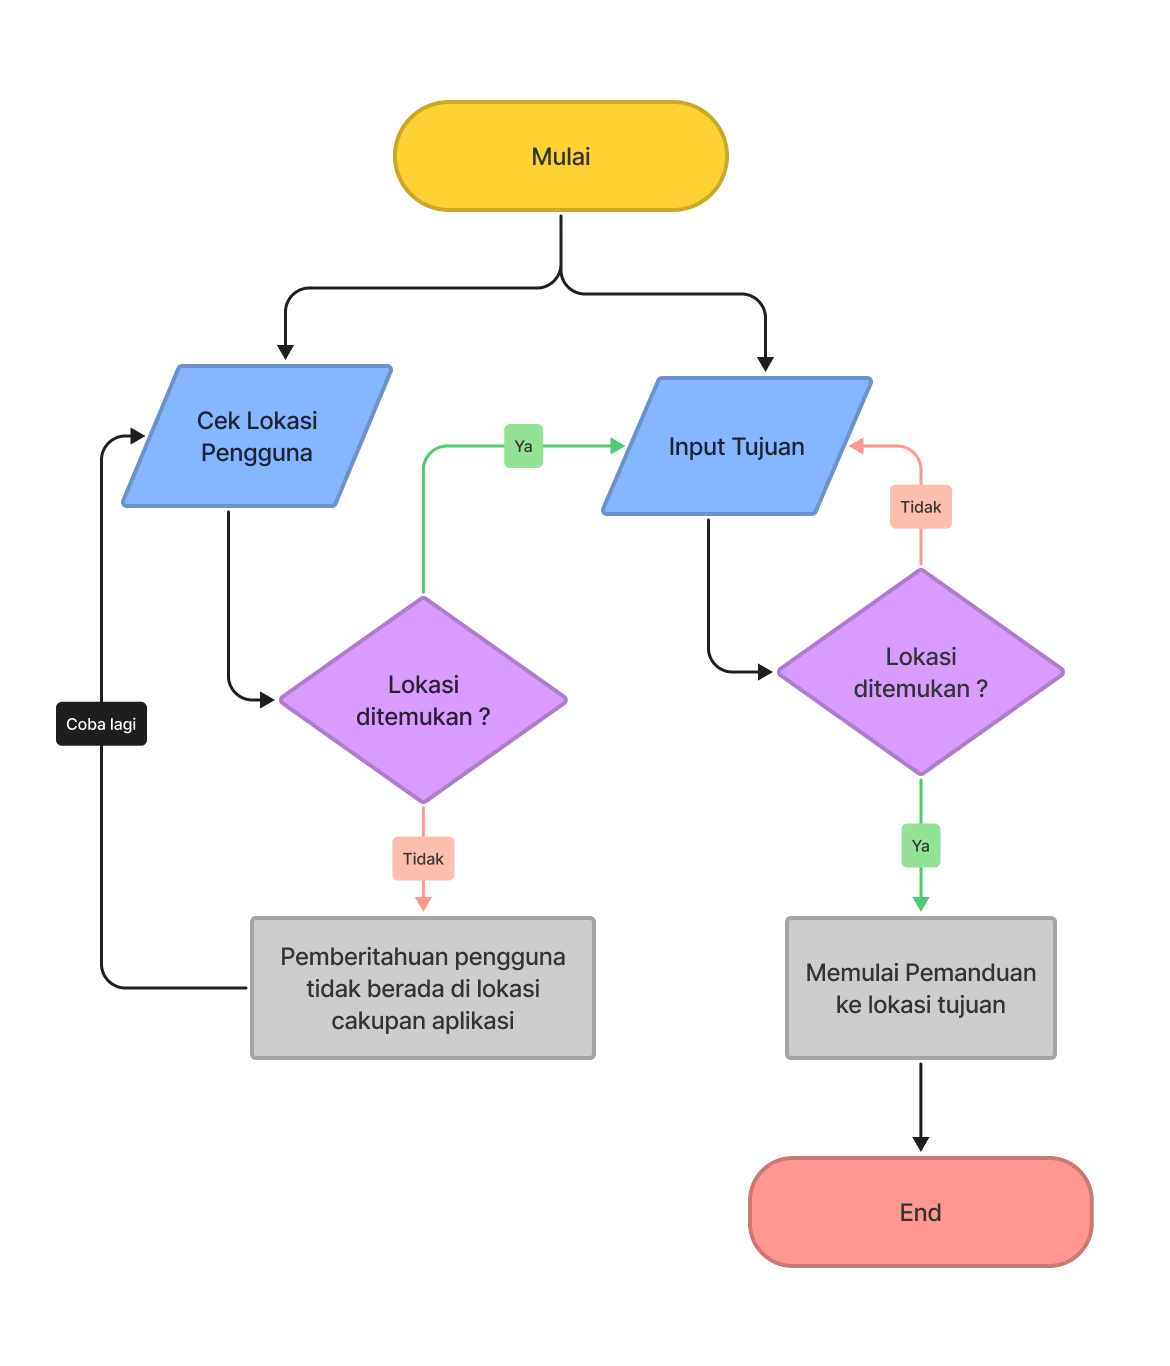
\includegraphics [scale = 0.35]{gambar/bab3/flow_diagram_app}}
\caption{\textit{Flow Diagram} Navigasi \textit{Indoor}}
\label{img:flow_diagram_app}
\end{figure}

\item Desain Prototipe
\par Desain prototipe menunjukkan perkiraan tampilan aplikasi yang akan dibuat. Desain ini dirancang berdasarkan beberapa skenario pada sisi pengguna baik tunanetra dan bukan tunanetra.

\vspace{-0cm}
	\begin{figure} [H]
	\begin{subfigure}{.5\textwidth}
  		\centering
  		% include first image
  		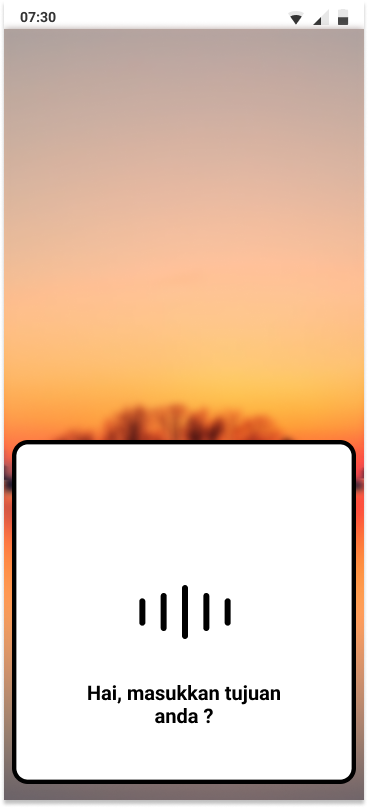
\includegraphics[width=.5\linewidth]{gambar/bab3/1}  
  		\caption{Pop up trigger by hotword}
	\end{subfigure}
	\begin{subfigure}{.5\textwidth}
  		\centering
  		% include second image
		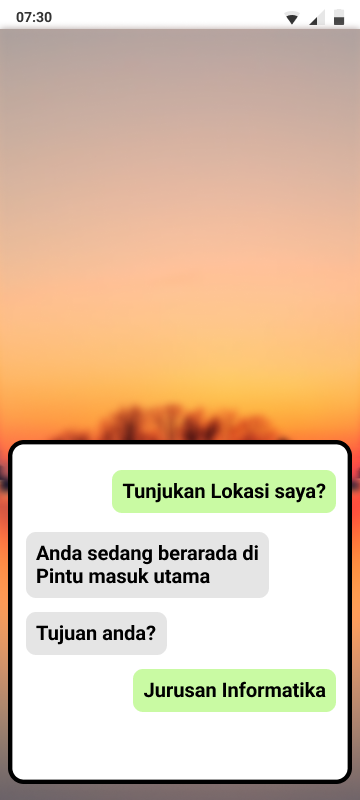
\includegraphics[width=.5\linewidth]{gambar/bab3/2}  
  		\caption{Input tujuan dan lokasi pengguna}
	\end{subfigure}
		\vspace{1cm}
		\newline
	\begin{subfigure}{.5\textwidth}
  		\centering
		 % include third image
	  	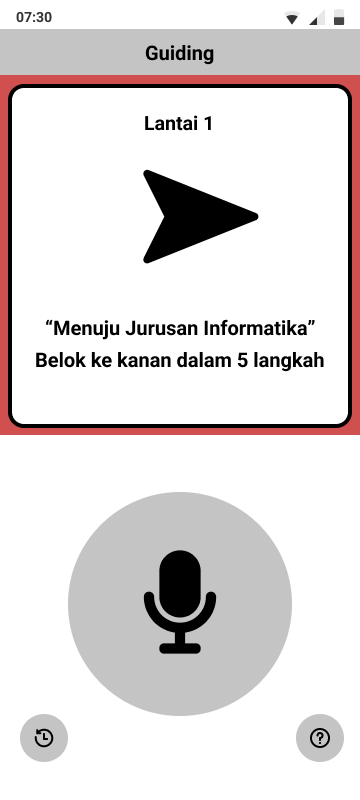
\includegraphics[width=.5\linewidth]{gambar/bab3/3}  
  		\caption{Proses Navigasi ke Tujuan}
	\end{subfigure}
	\begin{subfigure}{.5\textwidth}
  		\centering
  		% include fourth image
  		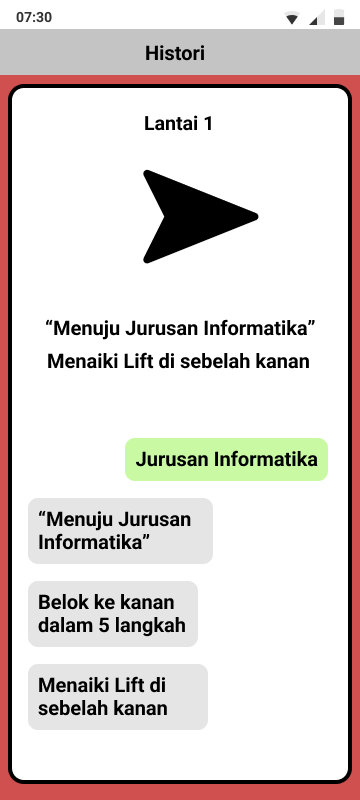
\includegraphics[width=.5\linewidth]{gambar/bab3/4}  
  		\caption{Histori Navigasi}
	\end{subfigure}
		\vspace{0.5cm}
		\caption{Tampilan Halaman Aplikasi Navigasi Indoor untuk Tunanetra}
	\label{aplikasimappingbagian1}
	\end{figure}

\end{enumerate}


\newpage

\section{Pembuatan Sistem}
\subsection{Persiapan data}

	\begin{enumerate}
	\item Data Model \textit{Voice Recognition}
	\par Data yang digunakan dalam penelitian ini terdiri atas data \textit{pre-trained} model yang diperoleh dari penelitian yang berada dalam satu penelitian yang sama pada \textit{roadmap} pada gambar \ref{img:fase2}. \textit{Pre-trained} model dimanfaatkan sebagai titik awal untuk merespons perintah suara dari pengguna, kemudian perintah suara akan di terjemahkan ke dalam bentuk teks yang akan diterima oleh \textit{smartphone} pengguna. Teks yang diterima akan digunakan sebagai input yang akan menjadi lokasi tujuan serta pemilihan rute. Berikut adalah \textit{list} dari nama-nama ruangan yang ada pada data \textit{Pre-trained} model.

% Please add the following required packages to your document preamble:
% \usepackage{multirow}
% \usepackage{longtable}
% Note: It may be necessary to compile the document several times to get a multi-page table to line up properly
\begin{longtable}[c]{|l|l|c|}
\caption{Data Ruangan \& Perintah}
\label{t_data}\\
\hline
\textbf{No.} & \textbf{Nama Ruangan}          & \multicolumn{1}{l|}{\textbf{Keterangan}} \\ \hline
\endfirsthead
%
\multicolumn{3}{c}%
{{\bfseries Table \thetable\ continued from previous page}} \\
\endhead
%
1            & ruang cctv                     & \multirow{6}{*}{Lantai 1}                \\ \cline{1-2}
2.           & ruang kepegawaian              &                                          \\ \cline{1-2}
3.           & ruang tata usaha               &                                          \\ \cline{1-2}
4.           & ruang tu                       &                                          \\ \cline{1-2}
5.           & ruang kemahasiswaan            &                                          \\ \cline{1-2}
6.           & ruang akademik                 &                                          \\ \hline
7.           & ruang dekan                    & \multirow{7}{*}{Lantai 2}                \\ \cline{1-2}
8.           & ruang wakil dekan satu         &                                          \\ \cline{1-2}
9.           & ruang wd satu                  &                                          \\ \cline{1-2}
10.          & ruang wakil dekan dua          &                                          \\ \cline{1-2}
11.          & ruang wd dua                   &                                          \\ \cline{1-2}
12.          & ruang wakil dekan tiga         &                                          \\ \cline{1-2}
13.          & ruang wd tiga                  &                                          \\ \hline
14.          & jurusan informatika            & \multirow{18}{*}{Lantai 3}               \\ \cline{1-2}
15.          & jurusan d tiga mi              &                                          \\ \cline{1-2}
16.          & jurusan farmasi                &                                          \\ \cline{1-2}
17.          & ruang seminar                  &                                          \\ \cline{1-2}
18.          & laboratorium jaringan komputer &                                          \\ \cline{1-2}
19.          & lab jaringan komputer          &                                          \\ \cline{1-2}
20.          & laboratorium jaringan          &                                          \\ \cline{1-2}
21.          & lab jaringan                   &                                          \\ \cline{1-2}
22.          & laboratorium jarkom            &                                          \\ \cline{1-2}
23.          & lab jarkom                     &                                          \\ \cline{1-2}
24.          & laboratorium basis data        &                                          \\ \cline{1-2}
25.          & lab basis data                 &                                          \\ \cline{1-2}
26.          & laboratorium data mining       &                                          \\ \cline{1-2}
27.          & lab data mining                &                                          \\ \cline{1-2}
28.          & laboratorium multimedia        &                                          \\ \cline{1-2}
29.          & lab multimedia                 &                                          \\ \cline{1-2}
30.          & laboratorium gis               &                                          \\ \cline{1-2}
31.          & lab gis                        &                                          \\ \hline
32.          & mushala                        & \multirow{25}{*}{Ruangan Umum}           \\ \cline{1-2}
33.          & surau                          &                                          \\ \cline{1-2}
34.          & tempat shalat                  &                                          \\ \cline{1-2}
35.          & toilet wanita                  &                                          \\ \cline{1-2}
36.          & toilet pria                    &                                          \\ \cline{1-2}
37.          & toilet perempuan               &                                          \\ \cline{1-2}
38.          & toilet laki laki               &                                          \\ \cline{1-2}
39.          & toilet cewek                   &                                          \\ \cline{1-2}
40.          & toilet cowok                   &                                          \\ \cline{1-2}
41.          & kamar mandi perempuan          &                                          \\ \cline{1-2}
42.          & kamar mandi wanita             &                                          \\ \cline{1-2}
43.          & kamar mandi cewek              &                                          \\ \cline{1-2}
44.          & kamar mandi pria               &                                          \\ \cline{1-2}
45.          & kamar mandi laki laki          &                                          \\ \cline{1-2}
46.          & kamar mandi cowook             &                                          \\ \cline{1-2}
47.          & wc perempuan                   &                                          \\ \cline{1-2}
48.          & wc wanita                      &                                          \\ \cline{1-2}
49.          & wc cewek                       &                                          \\ \cline{1-2}
50.          & wc pria                        &                                          \\ \cline{1-2}
51.          & wc laki laki                   &                                          \\ \cline{1-2}
52.          & wc cowok                       &                                          \\ \cline{1-2}
53.          & pintu masuk                    &                                          \\ \cline{1-2}
54.          & pintu utama                    &                                          \\ \cline{1-2}
55.          & pintu masuk utama              &                                          \\ \cline{1-2}
56.          & pintu keluar                   &                                          \\ \hline
\end{longtable}


	\newpage
	
	\item Data Rute dan Denah Lokasi Penelitian
	\par Rute yang akan digunakan berlokasi di gedung A FMIPA lantai 1 sampai dengan lantai 3. Data rute yang digunakan akan dipetakan dengan menggunakan bantuan BLE. Data titik-titik BLE disimpan dalam \textit{database} lokal berupa MAC \textit{Address}, nilai RSSI, dan nama perangkat BLE. BLE berjumlah 40 unit dengan BLE untuk ruangan berjumlah 25 ditandai dengan titik berwarna hijau dan BLE untuk \textit{connector} berjumlah 15 ditandai dengan titik berwarna biru.Jarak masing-masing BLE berada di sekitar 3 s/d 8 meter dari masing-masing BLE mengikuti jarak antara ruangan. Denah lokasi penelitian dapat dilihat pada gambar berikut.
	
	\begin{figure}[H]
\centering
{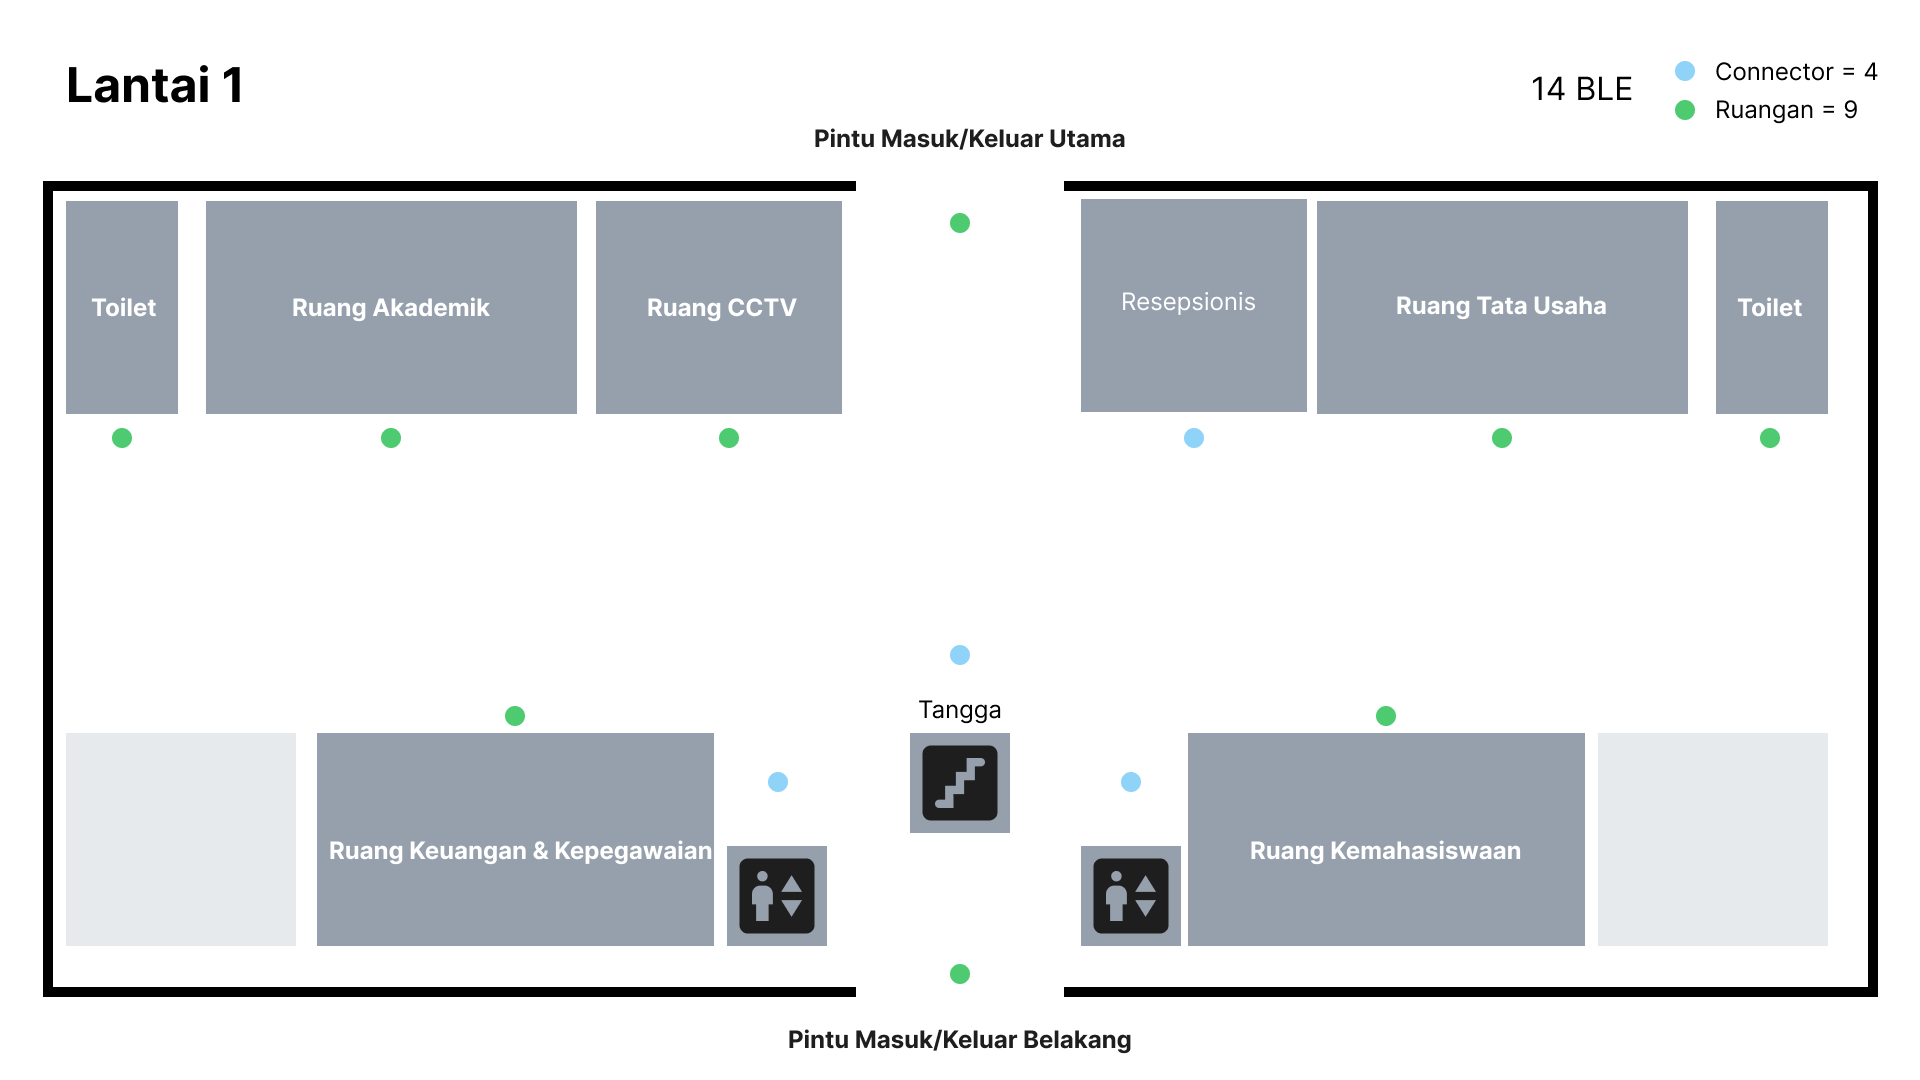
\includegraphics [scale = 0.2]{gambar/bab4/Denah-1-BLE}}
\caption{Denah lantai 1 Gedung A FMIPA dengan BLE}
\label{img:denah_1_ble}
\end{figure}

\begin{figure}[H]
\centering
{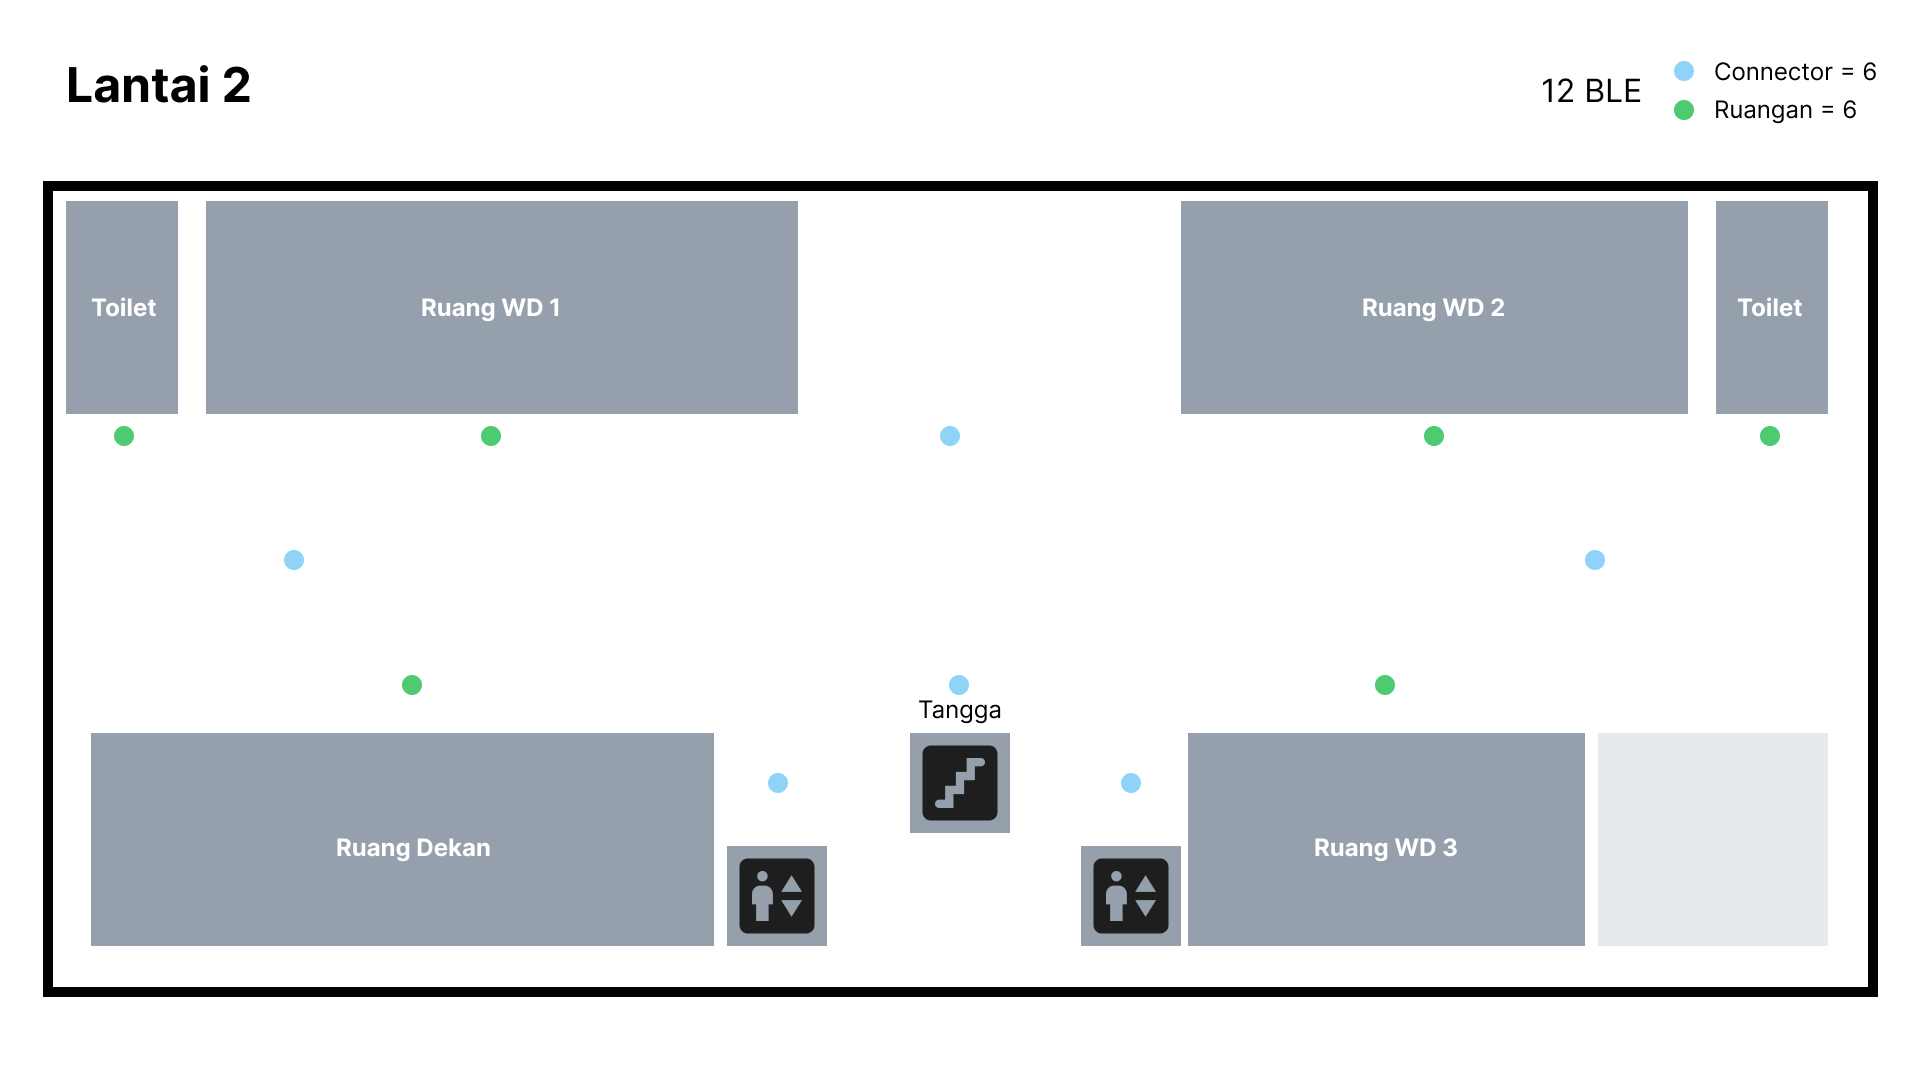
\includegraphics [scale = 0.2]{gambar/bab4/Denah-2-BLE}}
\caption{Denah lantai 2 Gedung A FMIPA dengan BLE}
\label{img:denah_2_ble}
\end{figure}

\begin{figure}[H]
\centering
{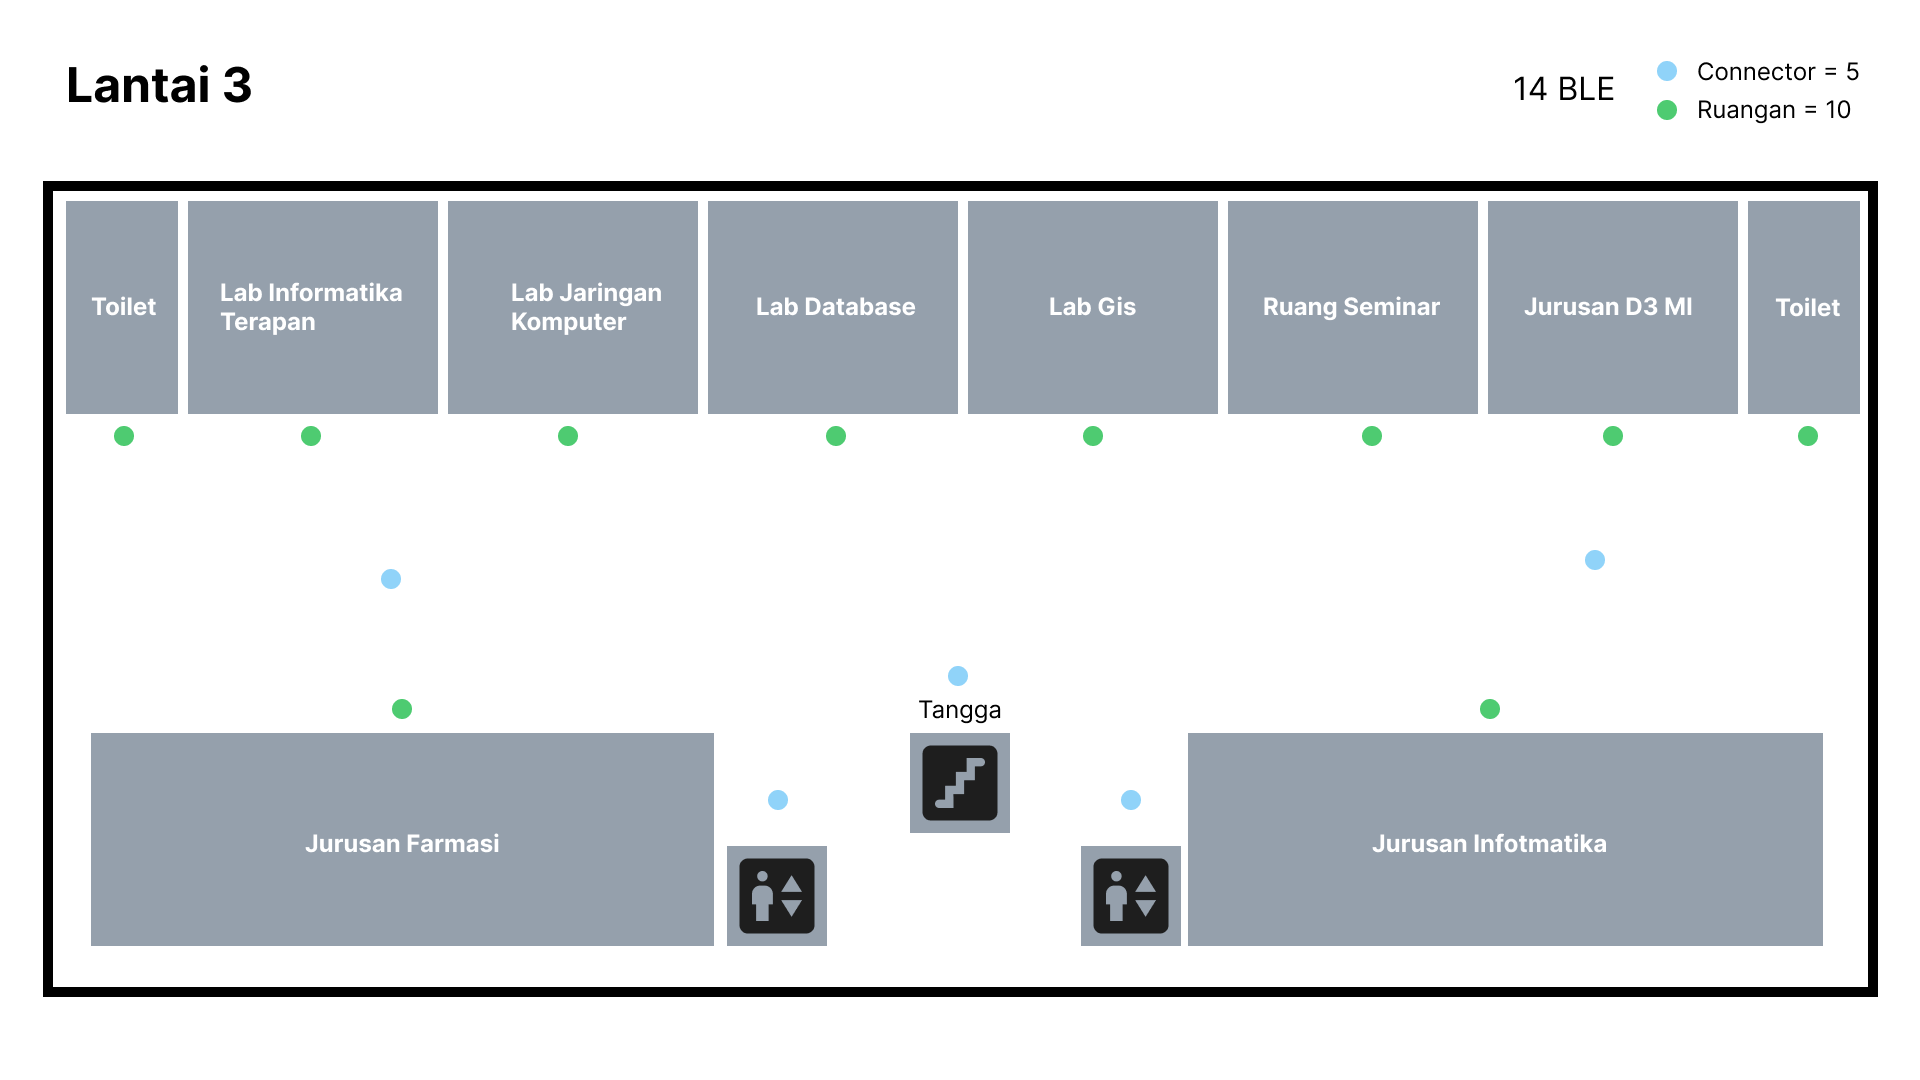
\includegraphics [scale = 0.2]{gambar/bab4/Denah-3-BLE}}
\caption{Denah lantai 3 Gedung A FMIPA dengan BLE}
\label{img:denah_3_ble}
\end{figure}
    
	\end{enumerate}
	
	
	
\subsection{Pembuatan Aplikasi}

	\begin{enumerate}
	
	\item Konfigurasi Model \textit{Voice Recognition} dan \textit{Text-to-speech}
	\par Pada tahapan ini model dipasangkan ke dalam aplikasi dengan menggunakan VOSK API dan Google \textit{text-to-speech} dengan menggunakan fungsi Talkback pada Android sehingga aplikasi dapat menerima input dari pengguna serta memberikan informasi \textit{feedback} ke pengguna saat dipandu.
	
	\newpage
	\item  Data akurasi lokasi pengguna serta akurasi rute
\par Data yang akan diperoleh dari proses koneksi BLE terdekat dengan RSSI sebagai tolak ukur akurasi lokasi pengguna, sedangkan untuk akurasi rute menggunakan data pemetaan rute dan lokasi tujuan yang telah dipetakan pada aplikasi dengan memanfaatkan RSSI dari beberapa koneksi BLE terdekat yang saling terhubung menggunakan Kalman Filter.

	\item Pembuatan Aplikasi
	\par Aplikasi dibuat dengan menggunakan bahasa pemrograman Kotlin dengan menggunakan \textit{jetpack compose} melalui IDE Android Studio. Media penyimpanan data BLE dan lokasi menggunakan basis data ROOM. Basis data disimpan secara lokal dan dapat diakses menggunakan query MySQL berbasis DAO ROOM. BLE dan data lokasi tersimpan berupa Id, RSSI, MAC Address, nama ruangan. Proses input pengguna dapat memanggil aplikasi secara langsung menggunakan suara dan memberi lokasi tujuan. Titik mulai pengguna diakses menggunakan Bluetooth dengan mencari BLE terdekat dengan lokasi pengguna.
	
	\vspace{-0cm}
	\begin{figure} [H]
	\begin{subfigure}{.5\textwidth}
 		\centering
 		% include first image
 		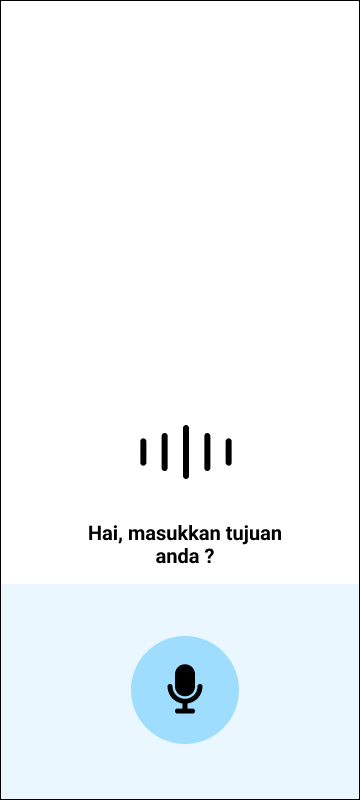
\includegraphics[width=.5\linewidth]{gambar/bab4/pandu-pop-up} 
 		\caption{Pop up trigger by hotword}
	\end{subfigure}
	\begin{subfigure}{.5\textwidth}
 		\centering
 		% include second image
		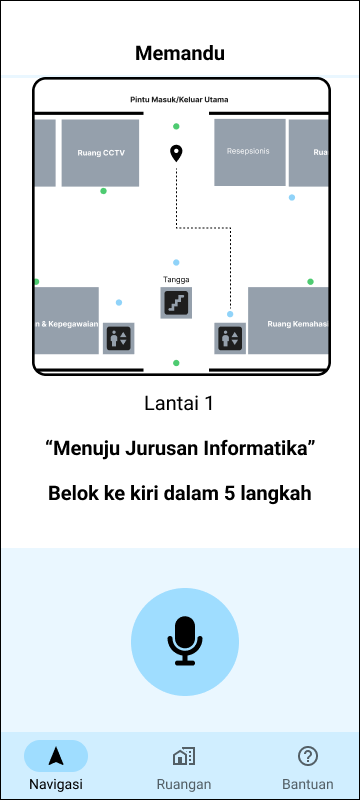
\includegraphics[width=.5\linewidth]{gambar/bab4/memandu} 
 		\caption{Input tujuan dan lokasi pengguna}
	\end{subfigure}
		\vspace{1cm}
		\newline
	\begin{subfigure}{.5\textwidth}
 		\centering
		 % include third image
	  	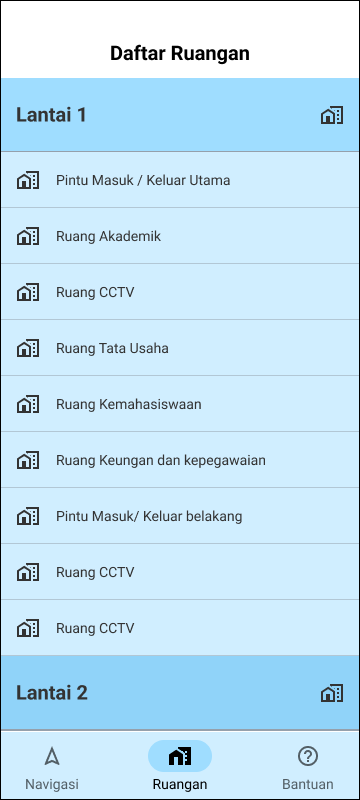
\includegraphics[width=.5\linewidth]{gambar/bab4/daftar-ruangan} 
 		\caption{Daftar Ruangan}
	\end{subfigure}
	\begin{subfigure}{.5\textwidth}
 		\centering
 		% include fourth image
 		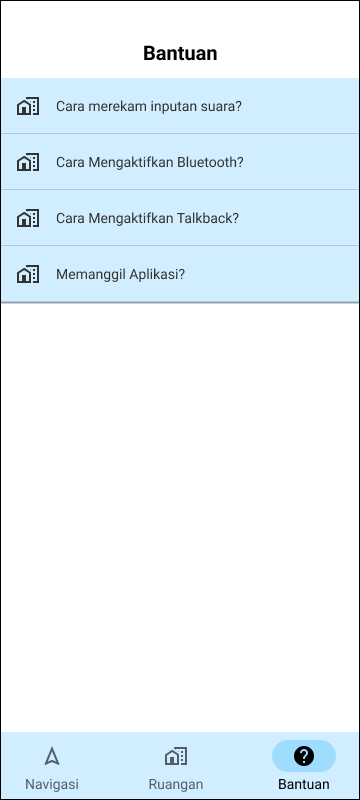
\includegraphics[width=.5\linewidth]{gambar/bab4/bantuan} 
 		\caption{Bantuan}
	\end{subfigure}
		\vspace{0.5cm}
		\caption{Tampilan Halaman Aplikasi Navigasi Indoor untuk Tunanetra}
	\label{aplikasimappingbagian1}
	\end{figure}

\end{enumerate}

\newpage
\section{Pengujian Sistem}
\subsection{Akurasi rute}
\par Pengujian akurasi posisi dan rute pengguna menggunakan gabungan titik BLE terdekat dengan mengukur kekuatan RSSI, kemudian menggunakan letak dan posisi BLE yang telah dipetakan dengan menghitung menggunakan Kalman Filter yang disertai dengan pembaharuan prediksi titik lokasi pengguna ke tujuan dan menghingtung kesalahan prediksi dan estimasi dengan data aktual.
Pengujian menggunakan 3 skema pengujian yang di uji pada 5 pengguna tunanetra seperti pada Tabel \ref{tab:skema-pengujian} berikut




\begin{table}[H]
\caption{Skema Pengujian Akurasi Pengambilan Rute di Gedung A FMIPA Optimal dalam MSE \textit{(Mean Squared Error)}}
\label{tab:skema-pengujian}
\resizebox{\columnwidth}{!}{
\begin{tabular}{|c|c|c|c|c|c|c|c|c|}
\hline
\textbf{No.} & \textbf{Titik Awal} & \textbf{Tujuan} & \textbf{Pengguna 1} & \textbf{Pengguna 2} & \textbf{Pengguna 3} & \textbf{Pengguna 4} & \textbf{Pengguna 5} & \textbf{Rute Optimal} \\ \hline
1 & Pintu masuk utama   & Toilet lantai 1     & 1.252 & 10.254 & 3.325 & 2.902 & 0.873 & 0.577 \\ \hline
2 & Pintu masuk utama   & Jurusan Informatika & 4.213 & 6.321  & 3.126 & 4.234 & 5.432 & 2.332 \\ \hline
3 & Jurusan Informatika & Pintu Keluar Utama  & 5.432 & 4.213  & 6.783 & 5.126 & 4.786 & 2.213 \\ \hline
\end{tabular}
}
\end{table}

\par Data Aktual berupa data pengembang dengan menggunakan perhitungan jarak BLE berdasarkan jarak antar BLE dan tujuan akhir secara langsung secara berurut mengikuti BLE terdekat, didapati MSE \textit{(Mean Squared Error)} seperti pada Tabel \ref{tab:skema-pengujian}. Terdapat pengguna mendapati rute yang mendekati rute optimal yang dipilih oleh aplikasi, sehingga pengguna yang mendekati rute optimal memiliki MSE rendah yang berarti mendekati akurat. Terdapat juga pengguna yang memiliki MSE tinggi dapat dipengaruhi oleh beberapa faktor seperti sinyal BLE, lokasi BLE, tembok, lokasi pengguna, dan saran rute yang diberikan melewati rute yang jauh dari rute optimal.

\newpage
\subsection{Pengujian Usabilitas UMUX}
\par Pengujian usabilitas bertujuan untuk menguji kelayakan dan kegunaan dari sistem yang akan digunakan oleh pengguna. Sebelum pengujian ini dilakukan, adapun skema pengujian yang telah dibuat dapat dilihat pada Tabel \ref{tab:skema-pengujian}.

\par Pengujian dengan metode UMUX dilakukan dengan menanyakan pertanyaan kepada responden. Kuesioner berisi 4 pertanyaan dengan menggunakan skala 1-7. Hasil pengujian UMUX aplikasi dapat dilihat pada Tabel \ref{tab:skor-umux} berikut.

% Please add the following required packages to your document preamble:
% \usepackage{multirow}
\begin{table}[H]
\caption{Hasil Pengujian UMUX Aplikasi Navigasi}
\label{tab:skor-umux}
\centering
\begin{tabular}{|ccccc|c|}
\hline
\multicolumn{1}{|c|}{\multirow{2}{*}{\textbf{Responden}}} & \multicolumn{4}{c|}{\textbf{Kode Pertanyaan}} & \multirow{2}{*}{\textbf{Skor UMUX}} \\ \cline{2-5}
\multicolumn{1}{|c|}{}  & \multicolumn{1}{c|}{U1} & \multicolumn{1}{c|}{U2} & \multicolumn{1}{c|}{U3} & U4 &       \\ \hline
\multicolumn{1}{|c|}{1} & \multicolumn{1}{c|}{6}  & \multicolumn{1}{c|}{2}  & \multicolumn{1}{c|}{7}  & 3  & 83,33 \\ \hline
\multicolumn{1}{|c|}{2} & \multicolumn{1}{c|}{5}  & \multicolumn{1}{c|}{3}  & \multicolumn{1}{c|}{5}  & 2  & 70,83 \\ \hline
\multicolumn{1}{|c|}{3} & \multicolumn{1}{c|}{7}  & \multicolumn{1}{c|}{2}  & \multicolumn{1}{c|}{6}  & 2  & 87,5  \\ \hline
\multicolumn{1}{|c|}{4} & \multicolumn{1}{c|}{5}  & \multicolumn{1}{c|}{2}  & \multicolumn{1}{c|}{4}  & 2  & 70,83 \\ \hline
\multicolumn{1}{|c|}{5} & \multicolumn{1}{c|}{5}  & \multicolumn{1}{c|}{2}  & \multicolumn{1}{c|}{6}  & 2  & 79,16 \\ \hline
\multicolumn{5}{|c|}{Rata-Rata}                                                                            & 78,33       \\ \hline
\end{tabular}
\end{table}

\par Berdasarkan hasil pengujian UMUX yang telah dilakukan diatas hasil rata-rata pengujian Aplikasi ini mendapatkan skor sebesar 78,33\%. Dapat dilihat bahwa aplikasi yang telah dibangun memiliki skor interpretasi \textbf{"dapat diterima"}, seperti pada gambar \ref{img:umux_to_sus} berikut.

\begin{figure}[H]
\centering
{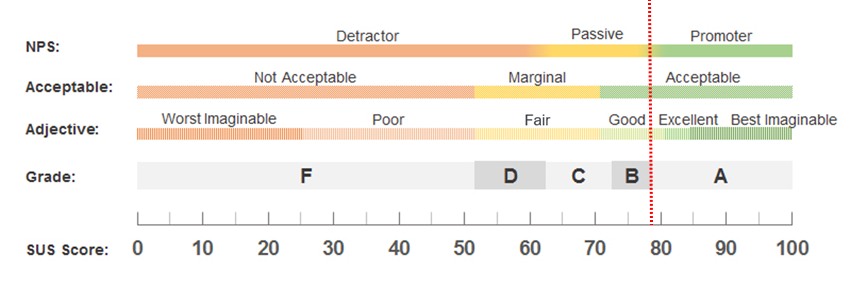
\includegraphics [scale = 0.5]{gambar/bab4/umux-to-sus}}
\caption{Skor UMUX ke SUS}
\label{img:umux_to_sus}
\end{figure}


\newpage
\subsection{Pengujian Fungsionalitas Menggunakan BlackBox}
\par Pengujian \textit{Blackbox} dilakukan dengan tujuan untuk menguji fungsionalitas dari aplikasi dengan menjalankan aplikasi tersebut apakah sesuai dengan alur bisni yang diinginkan.  Pengujian ini melihat fungsi yang tidak sesuai pada aplikasi dan
kesalahan-kesalahan aplikasi dalam mengerjakan suatu perintah. Fitur aplikasi yang diuji dapat dilihat pada Tabel \ref{tab:blackbox}.

\begin{table}[H]
\caption{Pengujian Blackbox Aplikasi Navigasi}
\label{tab:blackbox}
\resizebox{\columnwidth}{!}{
\begin{tabular}{|l|l|l|l|l|}
\hline
\textbf{No.} &
  \textbf{Nama Pengujian} &
  \textbf{Skenario} &
  \textbf{Tampilan} &
  \textbf{Hasil} \\ \hline
1. &
  Menghidupkan Bluetooth. &
  \begin{tabular}[c]{@{}l@{}}Klik tombol Allow pada \\ notifikasi yang muncul.\end{tabular} &
  Bluetooth akan menyala. &
  Berhasil \\ \hline
2. &
  Menghidupkan TalkBack. &
  \begin{tabular}[c]{@{}l@{}}Klik tombol Allow pada \\ notifikasi yang muncul.\end{tabular} &
  TalkBack akan menyala. &
  Berhasil \\ \hline
3. &
  Menghidupkan Mikrofon. &
  \begin{tabular}[c]{@{}l@{}}Klik tombol Allow pada \\ notifikasi yang muncul.\end{tabular} &
  Mikrofon akan menyala. &
  Berhasil \\ \hline
4. &
  Melihat daftar ruangan. &
  Klik icon gedung. &
  Diarahkan ke halaman daftar ruangan. &
  Berhasil \\ \hline
5. &
  Melihat daftar bantuan. &
  Klik icon bantuan. &
  Diarahkan ke halaman Bantuan. &
  Berhasil \\ \hline
6. &
  \begin{tabular}[c]{@{}l@{}}Memanggil Aplikasi dengan\\  Hotword.\end{tabular} &
  \begin{tabular}[c]{@{}l@{}}Mengucapkan "Hai Pandu" \\ pada layar mana saja.\end{tabular} &
  Aplikasi terbuka dan siap memandu. &
  Berhasil \\ \hline
7. &
  Memeriksa lokasi pengguna. &
  \begin{tabular}[c]{@{}l@{}}Proses berjalan di belakang \\ layar.\end{tabular} &
  \begin{tabular}[c]{@{}l@{}}Notifikasi pengguna berada atau tidak\\ di lokasi.\end{tabular} &
  Berhasil \\ \hline
8. &
  Melihat Detail Ruangan. &
  \begin{tabular}[c]{@{}l@{}}Klik item pada halaman \\ ruangan.\end{tabular} &
  Diarahkan ke halaman detail ruangan. &
  Berhasil \\ \hline
9. &
  Proses memandu. &
  \begin{tabular}[c]{@{}l@{}}Klik icon mikrofon atau \\ mengucapkan "Hai Pandu"\\ lalu memasukkan tujuan.\end{tabular} &
  \begin{tabular}[c]{@{}l@{}}Dipandu menuju tujuan dengan navigasi\\ suara.\end{tabular} &
  Berhasil \\ \hline
10. &
  Melihat detail bantuan. &
  Klik item pada bantuan. &
  Diarahkan ke halaman detail ruangan. &
  Berhasil \\ \hline
11. &
  \begin{tabular}[c]{@{}l@{}}Pengecekan Lokasi yang\\ tersedia.\end{tabular} &
  \begin{tabular}[c]{@{}l@{}}Pengguna memasukkan\\ tujuan, proses pengecekkan\\ lokasi dan ruangan berjalan\\ di belakang layar.\end{tabular} &
  \begin{tabular}[c]{@{}l@{}}Notifikasi ruangan tersedia atau tidak,\\ pengguna berada pada lokasi penelitian\\ atau tidak.\end{tabular} &
  Berhasil \\ \hline
12. &
  \begin{tabular}[c]{@{}l@{}}Proses intrupsi untuk \\ pembatalan atau pergantian\\ tujuan lokasi ditengah proses\\ pemanduan.\end{tabular} &
  \begin{tabular}[c]{@{}l@{}}Pengguna memasukkan \\ tujuan, proses pengecekan\\ lokasi dan ruangan berjalan\\ di belakang layar.\end{tabular} &
  \begin{tabular}[c]{@{}l@{}}Aplikasi terbuka dan meminta masukkan\\ pengguna serta proses pemanduan akan\\ berjalan.\end{tabular} &
  Berhasil \\ \hline
\end{tabular}
}
\end{table}

\par Berdasarkan hasil Black Box Testing dari tabel diatas menunjukkan bahwa Aplikasi dapat berjalan dengan baik dibuktikan dengan "berhasil" pada kolom hasil pengujian masing-masing fitur yang dikerjakan.



%-----------------------------------------------------------------------------%

% Baris ini digunakan untuk membantu dalam melakukan sitasi
% Karena diapit dengan comment, maka baris ini akan diabaikan
% oleh compiler LaTeX.
\begin{comment}
\bibliography{daftar-pustaka}
\end{comment}
